\chapter{Implementing a Linux KVM TCB in Rust}
\label{sec:rewrite}

%We want to rewrite SeKVM in Rust.
%We first forward port SeKVM from 4.18 to 5.15, this is to use newer features
%e.g. LTO.
%Then we employ the two pass method.

%The goal of this work is to leverage Rust's safety features in a hypervisor TCB.
%Our Rust-based hypervisor, \rustsec{}, follows the design described in
%\autoref{sec:sekvmintro}, and is based upon the SeKVM implementation.

%The goal of this work is to create a secure hypervisor by leveraging Rust's
%safety features in its TCB.
%Our Rust-based hypervisor, \rustsec{}, is based upon the SeKVM implementation.
In the process of developing \rustsec{},
we first forward ported SeKVM from its original Linux 4.18 version to the
newest long term support version Linux 5.15 at the time of development.
Once the forward port of SeKVM to Linux 5.15 is done, we then rewrote the SeKVM
TCB \secore{} in Rust to create \rustcore{}, \rustsec{}'s TCB. This chapter
describes the challenges that arose when implementing a Rust-based KVM TCB for
Linux 5.15, and the techniques employed to solve them.

\section{Forward Porting SeKVM from Linux 4.18 to Linux 5.15}
The Linux kernel gained many new features between version 4.18 and 5.15,
including performance optimizations such as Link-Time-Optimization (LTO) and
energy aware scheduling. And new kernel security features including
\code{clang} shadow call stacks, branch target identification, control flow
integrity (CFI), ARM Memory Tagging Extension (MTE), ARM pointer
authentication, and randomized stack offset per system call.
By forward porting SeKVM from its original Linux kernel version 4.18 to 5.15,
the codebase can benefit from these advancements.

%to take advantage of various new kernel features, for
%example  for better performance, ARM Pointer Authentication (5.0), Energy Aware Scheduling (5.0)
%clang shadow call stack, branch target identification (5.8), MTE (5.10), clang CFI (5.13), randomized stack offset per syscall (5.13)

SeKVM is based on the mainline KVM ARM in NVHE mode, therefore, to forward port
it to a newer kernel version, Kernel functions called by SeKVM must be updated. For example,
the data cache flushing function \code{\_\_flush\_dcache\_area} is changed to
\code{dcache\_clean\_inval\_poc} in Linux 5.15.
All outdated functions and macros in the SeKVM codebase are updated.
Moreover, a new KVM mode pkvm \cite{pkvm} is added to mainline KVM ARM in Linux
5.11, we made sure the logic of SeKVM and pkvm is separated such that the two
modes of operation can coexist in the codebase. This is done by checking for
the kernel configuration at KVM initialization, if the configuration option for
SeKVM is set, pkvm will not be initialized.
Mainline KVM had also made the code that runs in ARM's hypervisor mode (EL2)
more self-contained. Symbols belonging to EL2 are isolated from kernel mode
symbols name-wise, a prefix \code{\_\_kvm\_nvhe\_} is prepended to all symbols
in EL2.
Parts of SeKVM that references symbols in the original NVHE KVM EL2 code then
must adjust how it references those symbols. The predefined helper macro
\code{CHOOSE\_NVHE\_SYM()} is used, it prepends the prefix (\code{\_\_kvm\_nvhe\_})
for referencing NVHE symbols so that it is not required to write
\code{\_\_kvm\_nvhe\_} every time the code references a NVHE symbol. This makes
our code cleaner and easier to maintain. For SeKVM symbols that
need to be referenced by the original NVHE KVM EL2 code, in this case, the helper
macro \code{KVM\_NVHE\_ALIAS()} is used, which creates an additional symbol referring to the
same piece of data as the input symbol whose name is prepended by the NVHE
prefix, enabling the NVHE KVM EL2 code to reference it.
Furthermore, to resolve the issue that the compiler optimizing struct zeroing
operations with \code{memset} calls, which are not mapped in EL2, the C
compiler flag \code{-ffreestanding} is included during the compilation of
SeKVM.

\section{Integrating Rust and Linux}

%challenge: Linux 5.15 does not include Rust support
%
%solution: our way of source code organization, build system integration,
%how we link Rust and C, data layout issues, etc.

In order to write a KVM TCB in Rust, Rust code must be compiled and linked with
the rest of the Linux kernel.
However, Linux 5.15, which is the latest long term support kernel version at
the time of \rustsec{} development, does not support Rust as a development
language. As a result, incorporating our Rust code into the kernel requires
the developer to manually invoke the Rust compiler to build the Rust crate, and
then link it against the kernel, which can be both laborious and susceptible to
errors.
To overcome this challenge, we integrated the Rust toolchain with the Linux
kernel build system. A new subdirectory in Linux's source path
\code{arch/arm64/krustvm} is created, and it contains the \rustcore{} crate
and the \code{Makefile} for this directory.
\rustcore{} is implemented in a single crate on the \code{no\_std} environment
and compiled into a single static library \code{libkrustvm.a}.
To support building \code{libkrustvm.a} and linking it with the
rest of the kernel with \code{make}, the following is added to the Makefile:
\begin{enumerate}
\item{append \code{libkrustvm.a} to Kbuild built-in object goals \code{obj-y} by adding the line \code{obj-y += libkrustvm.a}}
\item{define Makefile target
\begin{listing}[hbtp]
    \begin{minted}{Makefile}
$(obj)/libkrustvm.a: $(src)/krustvm/src/*.rs
        cargo build --release --target=aarch64-unknown-linux-gnu
    \end{minted}
    \label{lst:Makefile}
    \vspace{-1.2cm}
\end{listing}
to instruct \code{make} to use \code{cargo} to generate \code{libkrustvm.a}.
}
\item{convert \code{libkrustvm.a} into \code{krustvm.o} by calling \code{ld}}
\end{enumerate}
The Makefile in \code{arch/arm64/krustvm} generates \code{krustvm.o},
and the kernel build system will then link this file with all other object
files in the kernel and produce the final kernel image.

\section{Rewriting C-based \secore{} into Rust-based \rustcore{}}

%challenge: difficult to do a top-down design due to the difficulty to debug
%and complexity of a hypervisor (is this challenge kinda weak?)
%
%solution: two pass method, first function-by-function rewrite, then remove
%unsafe and redesign after we have a working Rust hypervisor, and leverage
%Rust to achieve a stronger memory region isolation guarantee.

\subsection{The Rewrite Process}
Given the high complexity of the KVM hypervisor and \secore{},
it is clear from the beginning that
a top-down approach to a Rust rewrite would be error-prone and difficult to test.
Therefore, we elected to start the rewriting effort bottom-up,
where all previous C functions in the TCB are rewritten in Rust, one by one.
This incremental approach allows us to test one rewritten function at a time,
reducing the risk of introducing bugs.
%One major downside of this approach is that it is difficult to rewrite a single
%function in a Rust-idiomatic and safe way.
One major downside of this approach is the difficulty of rewriting individual
functions in a manner that adheres to Rust's idiomatic practices, such as using
Rust's pattern-matching \code{match} syntax instead of the C-like \code{if}
statements, and using references instead of raw pointers.
Furthermore, it may result in a lot of \code{unsafe} blocks.
These issues are solved by adding a second phase to the Rust rewrite;
after the initial function by function rewrite, we removed unnecessary
\code{unsafe} blocks, refactored the code to be more Rust-idiomatic,
and leveraged Rust features to enhance \rustcore{} memory safety.
%We discuss the features used to secure \rustcore{} memory accesses in
%\autoref{sec:securercore}.

\subsection{Rust Code Organization}
\label{sec:RCO}

Rust packages code into \textit{modules}, modules are containers for functions,
types, constants, traits, etc. Rust programs or libraries are made up of one or
multiple modules.
\rustcore{} consists of multiple modules, including the typical utility
functions module, and modules that contain functions that implement different
hypervisor tasks, for example mapping a page in the host kernel's NPT.
%Moreover, there are modules that implement custom type definitions and their
%type methods.
Moreover, each of the \rustcore{} metadata types (\autoref{tab:metadata}) used
for storing NPT information, physical memory page ownership, VM information,
SMMU page table metadata, etc., is implemented as its own module that defines
the type and its associated type methods.
One of the modules is \code{VMInfo}, it includes the definition of the type
\code{VMInfo}, which stores information of a VM including its VMID, state, and
an array of VCPU states. The module also contains methods for reading the VMID,
setting the state of the VM, etc.
There is another module that aggregates the \rustcore{} metadata structures into a single big
structure \code{RcoreMetadata} (line 1 in \autoref{lst:rcoremetadata}) to simplify
the memory used by these metadata.
Some fields in \code{RcoreMetadata} are shared by all CPU cores, while others are per CPU.
We leverage the custom mutex type \code{\lock{}} from \cite{krustvmrepo} to
protect concurrent accesses to
fields shared by all CPU cores in \code{RcoreMetadata}.
Shared fields are defined as type \code{\lock{}<T>}
(an example is line 3 in \autoref{lst:rcoremetadata}),
where \code{T} is the type that actually stores \rustcore{} metadata.
\rustcore{}'s custom \code{\lock{}} is a generic type which can hold any
arbitrary type alongside a lock.
The only way to access the data wrapped in \code{\lock{}} is by calling the
\code{lock} method of \code{\lock{}} reference.
Different from Rust, C does not support methods for structs, it therefore lacks
the ability to present an API that provides type-specific functionalities while
hiding how the method's implementation manipulates the structure's data.
For instance in \autoref{lst:typemethod}, users of \code{VMInfo} is forbidden
from accessing the \code{vmid} field of \code{VMInfo} directly, but must call
the \code{get\_vmid} method. The user thus can not arbitrarily modify data
inside the structure. This Rust feature helps eliminate bugs such as writing to
read-only fields, and accessing fields that are not intended to be exposed to
the users of the type.

\begin{table}
\begin{tabular}{ |p{0.2\linewidth}|p{0.7\linewidth}| }
\hline
\footnotesize \textbf{Name} & \footnotesize \textbf{Decription of Data} \\ \hline
\footnotesize vCPU context & \footnotesize The array that stores the state of each vCPU register. \\ \hline
\footnotesize VM info & \footnotesize The per-VM execution state metadata. \\ \hline
\footnotesize NPT info & \footnotesize The NPT pool allocation status. \\ \hline
\footnotesize PMEM info & \footnotesize The physical memory ownership and sharing status. \\ \hline
\footnotesize SMMU info & \footnotesize The SMMU management and page tables metadata. \\ \hline
\footnotesize SMMUPT info & \footnotesize The SMMU page table pool allocation status. \\ \hline
\end{tabular}
\vspace{0.2cm}
\caption{\rustcore{} metadata}
\label{tab:metadata}
\vspace{-0.4cm}
\end{table}

\begin{listing}[ht]
    \begin{minted}{Rust}
struct RcoreMetadata {
  [...] // other fields omitted
  pub pmem_info: KMutex<PMemInfo>,
  [...] // other fields omitted
}

const RCORE_METADATA_PTR: *mut RcoreMetadata = /* Rcore's memory address */;

    \end{minted}
    \caption{\rustcore{} metadata}
    \label{lst:rcoremetadata}
    \vspace{-0.2cm}
\end{listing}

\begin{listing}[ht]
    \begin{minted}{Rust}
// in the VM module:
pub struct VMInfo {
    vmid: u32,
    [...] // other fields omitted
}

impl VMInfo {
    #[inline(always)]
    pub fn get_vmid(&self) -> u32 {
        self.vmid
    }
}
    \end{minted}
    \caption{type method example}
    \label{lst:typemethod}
    \vspace{-0.2cm}
\end{listing}

\subsection{Rust-Rewrite Challenges}
\textbf{Enforcing Linking Section.}
KVM separates EL2 code from EL1 by grouping EL2 code in a section
\code{.hyp.text}, then mapping that section in EL2's address space at
initialization.
In \rustcore{}, attribute \code{\#[link\_section = ".hyp.text"]} is prepended
to all code that should be run in EL2, so that they get placed in the
\code{.hyp.text} section as well.

\textbf{Matching Linux Types and Constants.}
Our implementation is compatible with the Linux kernel codebase. For example,
the page size definition is identical in \rustcore{} and KVM.
For types shared between Linux and \rustcore{} like \code{kvm\_vcpu}, the type
definitions are generated automatically with the tool
\code{bindgen}~\cite{bindgen}. \code{Bindgen} can generate Rust type
definitions by parsing C's struct definitions, saving developers' time that
would otherwise be spent defining the same type.
For types that are shared by both C and Rust, the Rust attribute
\code{\#[repr\-(C)]} is used to ensure their alignment, field layout order, and
padding are the same in both languages, to prevent data corruption. This
happens for example when the field layout of a structure is different for the
two languages, resulting in C and Rust accessing distinct offsets within the
structure when reading or writing to the same field.
And for constants that are used by both Linux
and \rustcore{}, including the page size mentioned above, they are copied from C
to Rust manually. Due to the limited support of macro in \code{bindgen} and its
complex usages by Linux, \code{bindgen} is not used to generate constants.

\textbf{Entry Point Binding.}
Whenever an exception gets taken to EL2, the CPU switches its exception level
to EL2, saves the program status and exception syndrome, and jumps to the
preassigned exception vector.
We modify the exception vectors, which are written in assembly, to call
\rustcore{}'s entry point functions instead of the original C handlers to
transfer the control flow to our Rust code.
\rustcore{}'s entry point functions must be annotated with the Rust attribute
\code{\#[no\_mangle]}. This attribute informs the Rust compiler that the
function name should not be mangled, in order for the linker to resolve the
symbol reference in the exception vectors.
%Rust functions in \rustcore{} are invoked in exception vectors.
%This is the place where our Rust code in \rustcore{} comes into play.
%The exception vectors are implemented in assembly, they call Rust
%exception handlers after it switches the register context to EL2.

\subsection{Unsafe Rust Usages}

A small part of \rustcore{}'s implementation is coded in unsafe Rust.
Unsafe Rust exists because the underlying computer hardware is inherently
unsafe. Certain tasks are impossible without unsafe operations, such as
directly accessing a specific address to configure the interrupt controller, or
issuing a memory barrier instruction in the middle of a function. Overall,
the source of unsafe Rust includes inline assembly, the Foreign Function
Interface (FFI), KVM ARM Per-CPU variables, and raw pointer accesses.
The first three categories are discussed in this section,
and for raw pointer usages, \autoref{sec:securercore} shows how each raw
pointer usage scenario is checked to guarantee their memory safety.

\textbf{Inline Assembly.}
Inline assembly are used for system instructions (e.g. TLB invalidation
instructions) and system register accesses.
ARM architecture uses the \code{mrs} instruction to read a system
register's value to a general purpose register, and the \code{msr} instruction
to write a system register with the content of a general purpose register.
Inline assembly can be inserted in Rust code with the help of Rust's built-in
\code{core::arch::asm} module. It can be used to embed handwritten assembly in
the assembly output generated by the compiler.
For system register accesses, the \code{aarch64-cpu} crate
\cite{aarch64cpu} is imported into our \rustcore{} crate, it provides a clean
API for reading and writing AArch64 system registers. The actual inline
assembly usages of \code{mrs} and \code{msr} are abstracted behind
\code{aarch64-cpu}'s safe APIs.

\textbf{FFI.}
FFIs are used for calling longer assembly routines, below is a list showing the FFI routines used in \rustcore{}.
\begin{itemize}
\item \code{\_\_guest\_enter}: context switching general purpose registers and entering guest VMs.
\item \code{dcache\_clean\_inval}: invalidate cache of the input memory range.
\item \code{acquire\_lock} and \code{release\_lock}: \rustcore{}'s spinlock primitive that spin on an address using an assembly loop.
\item \code{tlb\_flush\_ipa}: flushes the TLB of the input intermediate physical address range of the vmid given.
\end{itemize}

\textbf{KVM ARM Per-CPU Variables in Rust.}
Using KVM ARM Per-CPU variables is a special case for unsafe Rust.
Mainline KVM has its own EL2 per CPU variable mechanism (\autoref{fig:percpu});
it is implemented by first
allocating enough space for all cores to have a copy of the per CPU variables,
then, for each CPU core, it records the offset from its copy of the variables to the
base copy. This per-core offset is then stored in each core's \code{TPIDR\_EL2}
system register. When there is a requirement to access a per CPU variable, the
address of the base copy is first acquired, then \code{TPIDR\_EL2}'s value is
added to the base copy's address to calculate the per-core address.
\rustsec{} continues to use
this mechanism by declaring the symbol which corresponds to the base address as
a Rust extern static variable, take its raw address, then add the value in
\code{TPIDR\_EL2} to it. This approach requires three \code{unsafe} statements,
first from reading the address of the extern static variable, then reading
\code{TPIDR\_EL2} via inline assembly, and lastly, another \code{unsafe} to
dereference the calculated address. Concurrent accesses will not pose a problem
since each core accesses a different address.

\begin{figure}[hbtp]
    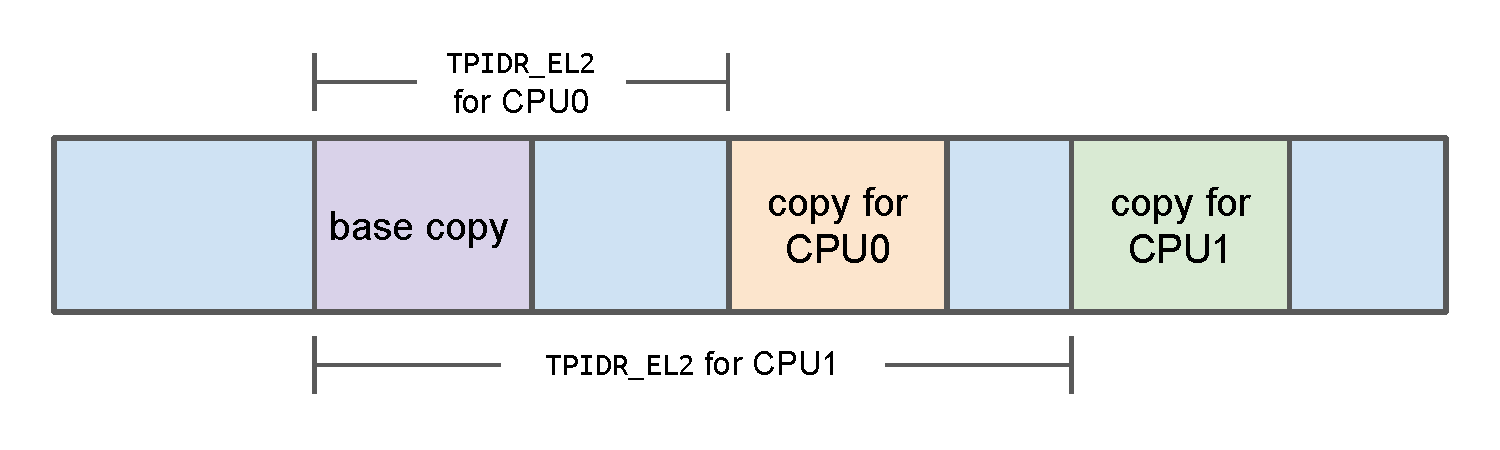
\includegraphics[scale=0.60]{figures/percpu.pdf}
    \caption{KVM ARM Per-CPU Variables Mechanism}
    \label{fig:percpu}
\end{figure}

\section{Bringing up \rustsec{} on Real Hardware}

We chose the Raspberry Pi model 4B (Rpi-4B) to verify our implementation on
real hardware.
%This section describes the problem that occured when trying to run SeKVM on
%Rpi-4B, and how we solved the issue.
SeKVM's trusted core \secore{} originally reserved its private memory by
defining global symbols whose addresses reside right after the kernel image,
in the Linux kernel linker script.
\secore{} then references those symbols to access and utilize the reserved
memory.
However, there is an unusable hole reserved for the GPU in the physical memory
address space of Rpi-4B, spanning from 948MB to 1GB. The proprietary bootloader
of Rpi-4B restricts the placement of the kernel image within the range of 0 to
948MB. Considering that SeKVM requires more than 1GB of private memory, an
overlap between \secore{}'s private memory and the unusable hole becomes
unavoidable (\autoref{fig:overlap}). This makes SeKVM unable to initialize on
Rpi-4B.

\begin{figure}[hbtp]
    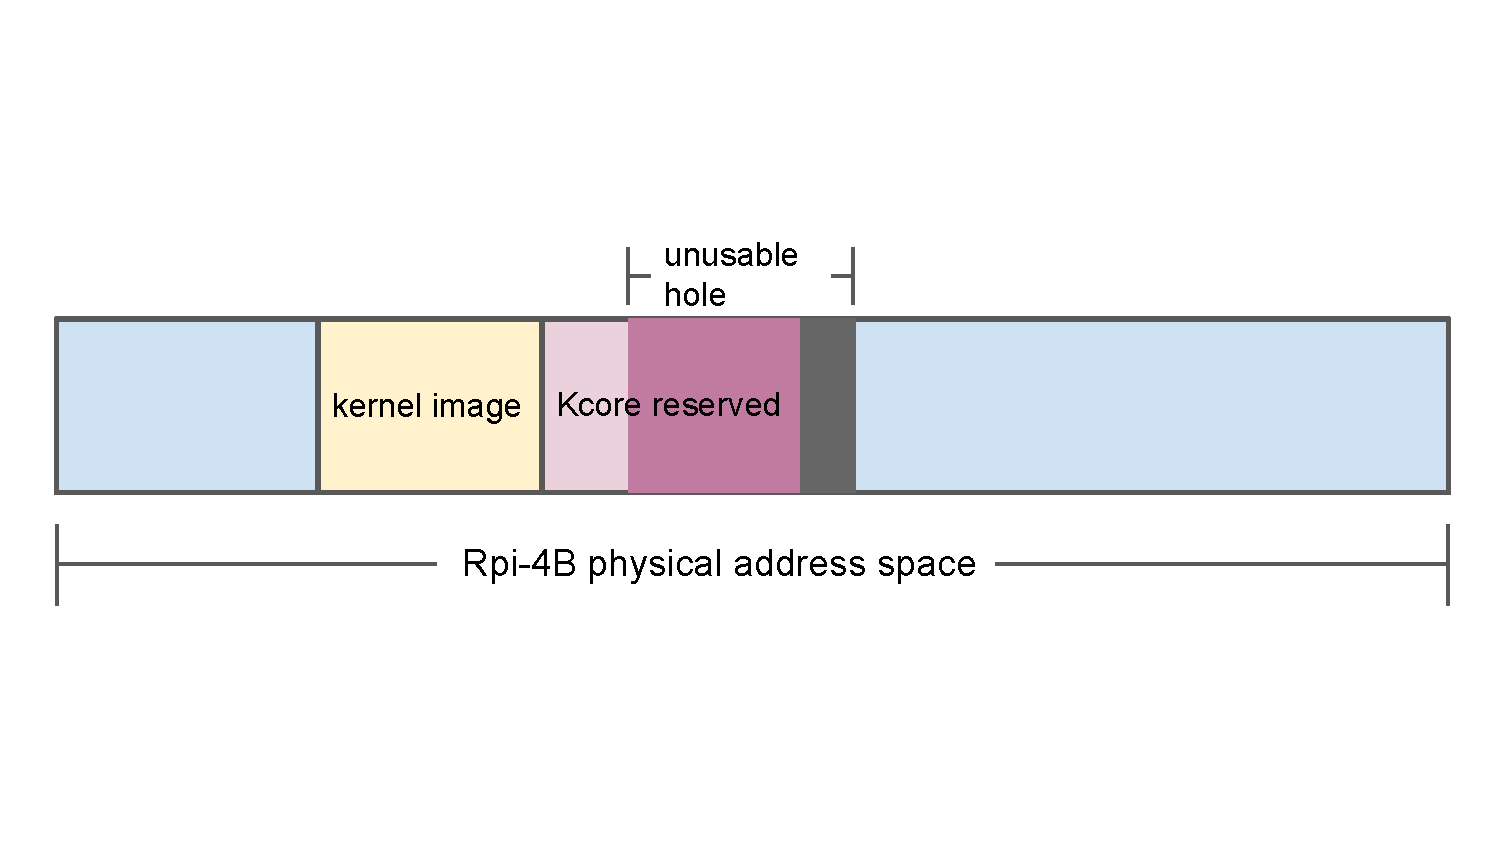
\includegraphics[scale=0.60]{figures/overlap.pdf}
    \caption{KCore overlaps the unusable hole on Rpi-4B}
    \label{fig:overlap}
\end{figure}

To solve this issue for \rustsec{}, instead of allocating memory in the linker
script, we first locate a range of memory which does not overlap with the
unusable hole of Rpi-4B and the kernel image, then add a new memblock that to
correspond to the \rustcore{}'s private memory. We mark it as reserved by
calling \code{memblock\_reserve}, so that the kernel does not accidentally
access this memory range (\autoref{fig:rcorereserved}). Malicious accesses to
\rustcore{} private memory from the host kernel are prevented by unmapping the
private memory from the host kernel's NPT.
%The global symbols previously defined the Linux kernel linker script have also
%been changed to macros that expand into addresses in the reserved range for
%\rustsec{}'s \rustcore{} usage.

\begin{figure}[H]
    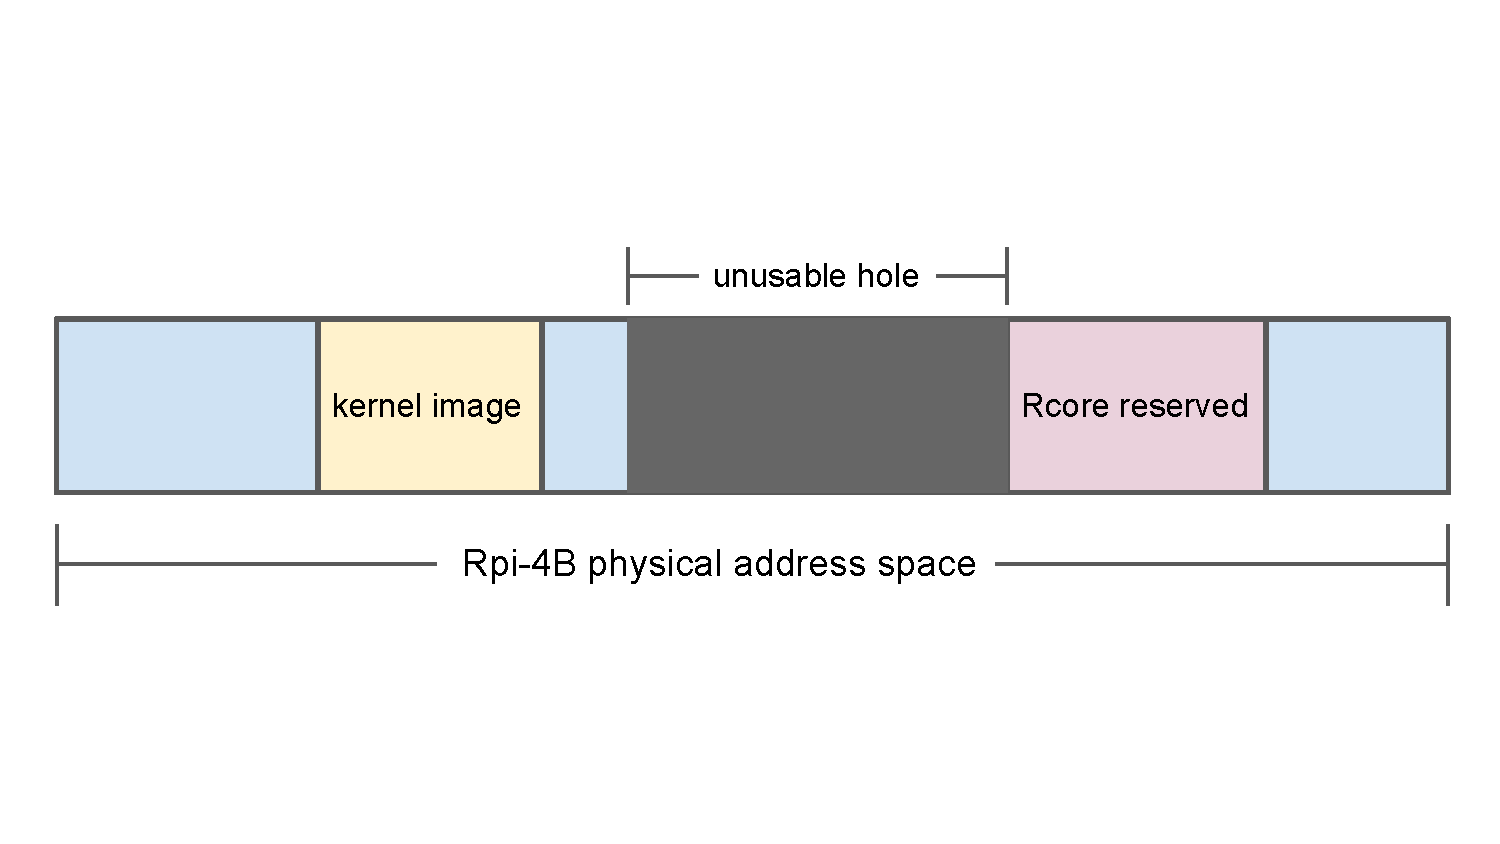
\includegraphics[scale=0.60]{figures/rcore_reserved.pdf}
    \caption{Overlap prevention}
    \label{fig:rcorereserved}
\end{figure}

